\documentclass[tikz]{standalone}
\usetikzlibrary{automata,positioning}
\begin{document}

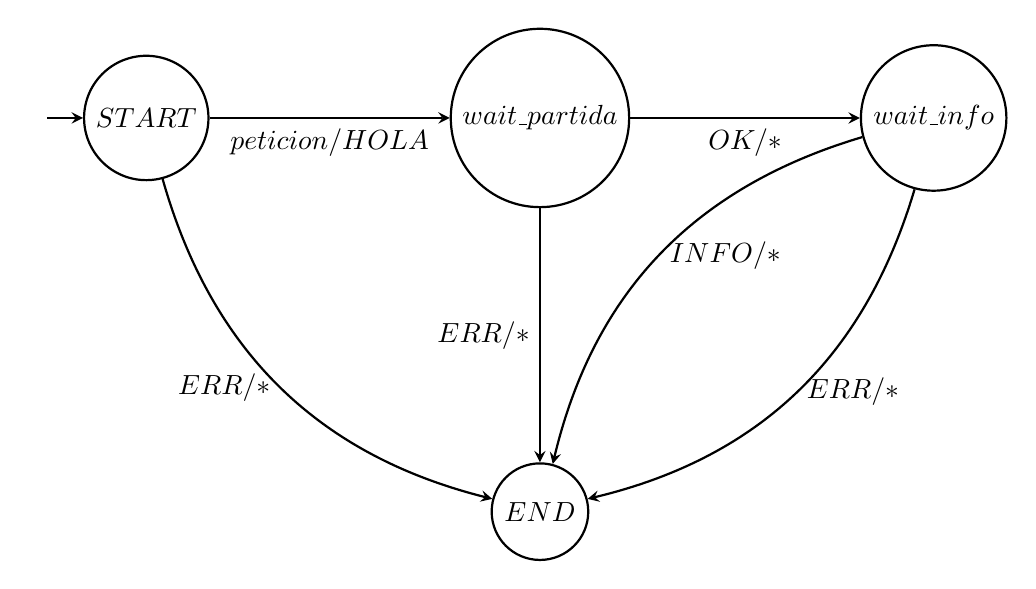
\begin{tikzpicture}[>=stealth,node distance=8cm,on grid,auto, thick, initial text=] 
  \node[state,initial] (q_0)   {$START$}; 
  \node[state]         (q_1) [right=5cm of q_0] {$wait\_partida$};
  \node[state]         (q_2) [right=5cm of q_1] {$wait\_info$};
  \node[state]         (q_3) [below=5cm of q_1] {$END$};

  \path[->]            (q_0) edge [bend right] node[left] {$ERR/*$} (q_3)
  					   (q_0) edge [right] node[below] {$peticion/HOLA$} (q_1)
  					   (q_1) edge [right] node[below] {$OK/*$} (q_2)
  					   (q_2) edge [bend right] node[right] {$INFO/*$} (q_3)
  					   (q_2) edge [bend left] node[right] {$ERR/*$} (q_3)
  					   (q_1) edge [below] node[left] {$ERR/*$} (q_3);
\end{tikzpicture}
\end{document}